\documentclass[conference]{IEEEtran}
\IEEEoverridecommandlockouts

\usepackage{cite}
\usepackage{amsmath,amssymb,amsfonts}
\usepackage{algorithmic}
\usepackage{graphicx}
\usepackage{textcomp}
\usepackage{xcolor}
\usepackage{kotex}
\def\BibTeX{{\rm B\kern-.05em{\sc i\kern-.025em b}\kern-.08em
    T\kern-.1667em\lower.7ex\hbox{E}\kern-.125emX}}
    
\begin{document}

\title{Connect to parent – FAFA\\ \LARGE(communicate tool for kids via voice recognition)}

\author{\IEEEauthorblockN{Park Hyeong Jin\\2016026271}
\IEEEauthorblockA{\textit{Dept. of Information System}\\ 
\textit{College of Engineering}\\
\textit{Hanyang University}\\
Seoul, Rep. of Korea\\
jin5378@hanyang.ac.kr}
\and
\IEEEauthorblockN{Lee Jun Seok\\2016026444}
\IEEEauthorblockA{\textit{Dept. of Information System}\\ 
\textit{College of Engineering}\\
\textit{Hanyang University}\\
Seoul, Rep. of Korea\\
junslee0912@gmail.com}
\and
\IEEEauthorblockN{Lee Jeong Seon\\2016026435}
\IEEEauthorblockA{\textit{Dept. of Information System}\\ 
\textit{College of Engineering}\\
\textit{Hanyang University}\\
Seoul, Rep. of Korea\\
com2769@gmail.com }
\and
\IEEEauthorblockN{Yoon Seung Gwon\\2016026371}
\IEEEauthorblockA{\textit{Dept. of Information System}\\ 
\textit{College of Engineering}\\
\textit{Hanyang University}\\
Seoul, Rep. of Korea\\
csyoon1472@gmail.com}
}

\maketitle

\begin{abstract}
FAFA is a parent-child connection service that is powered by artificial intelligence based voice recognition technology. The penetration rate of mobile phones among South Korea's senior elementary school students surpassed 90\% in 2018. However, the gap between the lower grade of elementary school(58.8\%) is too big, and it is expected to be bigger if in kids are included. In addition, the penetration rate of fixed-line telephones in households was 51.9\% in 2019, the lowest ever. Given the trend of these figures, two-way communication between parents and children under the lower grades of elementary school will become more difficult.

To solve this problem, we developed FAFA service which is based on voice recognition and web. The service tells parent’s location information for kid and sends message to parent that kid is looking for you. This service will enable two-way communication with parents and kids. 

\end{abstract}

\section{Introduction}
\subsection{Motivation}
Child Location Based Services (LBS), which is widely used by parent, is a child management service for parents. Parents who are concerned about their child’s safety check their child's current location through the LBS service.However, parents are not the only ones who are worried about their child, and their child wants to know where their parents are now and when they will come back home. Also, child who is left alone at home wants to communicate with his or her parents. We understood these demands and felt the need for a way to communicate child at home with parents.

\subsection{Problem statement (client’s needs)}
According to a report by the Korea Information Society Development Institute, the penetration rate of mobile phones in the lower grades children of elementary school in 2018 was 58.8\%. Including preschoolers, more than half of children under the age of 10 don't have cell phones. In addition, the penetration rate of landline phones in 2018 was 51.9\%.Parents are reluctant to buy their young children's cell phones for various reasons, including their children's addiction to smartphones and the burden of costs. When young children are alone at home, they often want to communicate with parents when they come to the house and where they are. However, Sometimes he can’t contact his parents due to the absence of communication means. In order to solve the demand for communication with young children and parents, we proposes a "parent-child connection" service that use NUGU speakers.

\subsection{Solution}
FAFA is a parent-child communication service by artificial Intelligence speech recognition technology of SKTelecom’s NUGU speaker. By using FAFA, Young child can communicate with their parents about where they are and when they will come back home. When the child asks the NUGU speaker where the parents are, it searches parent’s location and informs it. Also, When the child arrives at home and talks to the NUGU speaker, the alarm goes off on parent’s cell phone. The FAFA service uses NUGU speakers installed in the home to provide communication between parents and children at no additional cost.

\subsection{Research on any related software}
\begin{enumerate}
    \item iSharing Lifestyle\\
iSharing by iSharingSoft is an app that provides a real-time locator service allowing family members and close friends to privately share their location information and communicate with each other. iSharing help parents and caregivers reduce anxiety around the whereabouts of their loved ones with easy tracking and alerting messages. There are four main functions.
\begin{enumerate}
    \item Place alert : receive real-time alerts when family arrive at or leave destination
    \item Panic alert : Just shake phone to send notification messages to your family member
    \item Walkie-Talkie : Turn your phone into a Walkie-Talkie.
    \item Location History : See the location history of family member\\
\end{enumerate}
\item NUGU call\\
'NUGU-to-NUGU Call' is service about talking to your NUGU device or NUGU call subscriber.
This call is linked to data. You can use ‘normal mode’ to non NUGU call subscriber. A phone call is linked through the mobile phone of the account connected to the NUGU device.\\
\item NUGU SOS\\
 SOS service is that sends pre-set text messages to designated recipients. You can set the sender's and recipient's information and the emergency SOS message to be sent. If you request an emergency SOS to the NUGU speaker, we will send an emergency SOS message to your registered number.\\
 \item KAKAO mini\\
You can use Kakao Mini to send and read messages you received from users you want. Kakao Mini reads new messages from Kakao Talk's 1:1 chat room and group's Kakao Talk chat room. It reads messages from friends and reply. If it is not a text message, such as an emoticon or video, it tells the format of the message.
\end{enumerate}

\begin{table}[htbp]
\begin{center}
\caption{Role Assignments}
\begin{tabular}{|c|c|c|}
\hline
Roles & Name & Task description and etc \\ \hline
User  & \begin{tabular}[c]{@{}c@{}} Lee\\Jun Seok \end{tabular}& 
\begin{tabular}[c]{@{}c@{}}Predict what users need from the\\ perspective of a user. Also, consider\\ whether the service is easy to use and\\efficient to use.
If not, find the solution\\ and improve service quality.
\end{tabular}\\\hline

Customer&\begin{tabular}[c]{@{}c@{}}Lee\\Jeong Seon\end{tabular} &  
\begin{tabular}[c]{@{}c@{}}Analyze a service from the perspective\\of a buyer. Also, design service at an\\acceptable cost of money and resource,\\ and focus on cost-effectiveness\\ for raising purchase desire.  \end{tabular}\\ \hline

\begin{tabular}[c]{@{}c@{}}Software\\Developer\end{tabular}&
\begin{tabular}[c]{@{}c@{}}Park\\ Hyeong Jin\end{tabular}&
\begin{tabular}[c]{@{}c@{}}Design overall software to satisfy\\ users and customers' needs. Focus\\ on easiness of design, maintain, and\\reuse its parts.
  \end{tabular}\\ \hline

\begin{tabular}[c]{@{}c@{}}Development\\manger\end{tabular}&
\begin{tabular}[c]{@{}c@{}} Yoon\\Seung Gwon\end{tabular}&
\begin{tabular}[c]{@{}c@{}} Schedule overall project plan and\\ assign the tasks to the members.\\Try to sell more and please customers\\ while costing less to develop\\and maintain.  \end{tabular}\\ \hline  

\end{tabular}
\end{center}
\end{table}

\section{Requirements}
\subsection{AI Speaker (for kid)}
\begin{enumerate}
    \item Ask \& Answer parent’s location via voice
    \begin{enumerate}
        \item Set expected utterance that kid’s intent is asking parent’s location
        \item  Process parent’s location in backend proxy based on entity
        \item Get parent’s location and status. NUGU speaker will tell result using TTS function
    \end{enumerate}
    \item Send alert to parent
    \begin{enumerate}
        \item Send request to backend proxy when kids find their parents or tell speaker that they get home
        \item Server keep these request logs in database
    \end{enumerate}
    \item Inform that child has arrived home via voice
    \begin{enumerate}
        \item Set expected utterance that kid’s intent is informing that they arrived home
        \item Send request to backend proxy server
        \item Server keep request logs in database
    \end{enumerate}
\end{enumerate}

\subsection{Application (for parent)}
\begin{enumerate}
    \item Log-in
    \begin{enumerate}
        \item To identify users, token(user ID) is required
    \end{enumerate}
    \item Set location of home and company
    \begin{enumerate}
        \item To judge parent’s location and status, need to set longtitude and latitude of home and company
        \item User could set marker on map
    \end{enumerate}
    \item Update present location
    \begin{enumerate}
        \item Send present longtitude and latitude data to server
    \end{enumerate}
    \item View kid’s request log
    \begin{enumerate}
        \item Provide log of kid’s request in customized UI
    \end{enumerate}
\end{enumerate}

\subsection{Server}
\begin{enumerate}
    \item Judge parent’s location
    \begin{enumerate}
        \item Get parent’s location data from application
        \item Check latest location and judge status by customized algorithm
        \item Response to NUGU
    \end{enumerate}
    \item Send data to database
    \begin{enumerate}
        \item Server get data from NUGU speaker and application
        \item Server keep these data in database
    \end{enumerate}
    \item Make json for NUGU
    \begin{enumerate}
        \item Server should make json file. NUGU speaker demand data in REST API form\\
    \end{enumerate}
\end{enumerate}

\section{Development Environment}
\subsection{Software Development Platforms}
We chose native app to develop our project, and server acts as REST API. Web environment could also send location data, but we need more precise data and want it to be updated automatically. React Native which is front-end framework is used. Django which is back-end framework is used for developing REST API to connect with NUGU.

In addition, we will use AWS commercial cloud service such as Elastic Beanstalk for deploy. Lastly, SKT’s NUGU API will be used to analyze kids’ utterance and to recognize their intent.
\begin{enumerate}
    \item React Native\\
    React Native is a JavaScript framework for writing real, natively rendering mobile applications for iOS and Android. It’s based on React, Facebook’s JavaScript library for building user interfaces, but instead of targeting the browser, it targets mobile platforms. Similar to React for the Web, React Native applications are written using a mixture of JavaScript and XML-esque markup, known as JSX.\\
    \item Django (web framework)\\
    Django is a Python-based free and open source web framework that follows the model-template-views(MTV) architectural pattern. It is maintained by the Django Software Foundation. Django's primary goal is to ease the creation of complex, database-driven websites. The framework emphasizes reusability and "pluggability" of components, less code, low coupling, rapid development, and the principle of don't repeat yourself. Python is used throughout, even for settings files and data models.\\
    \item SQLite\\SQLite is a relational database management system (RDBMS) contained in a C library. In contrast to many other database management systems, SQLite is not a client–server database engine. Rather, it is embedded into the end program. SQLite is a popular choice as embedded database software for local/client storage in application software such as web browsers. It is arguably the most widely deployed database engine, as it is used today by several widespread browsers, operating systems, and embedded systems (such as mobile phones), among others. SQLite has bindings to many programming languages.\\
    \item Amazon Web Service Elastic Beanstalk(EB)\\
    AWS Elastic Beanstalk is an orchestration service offered by Amazon Web Services for deploying applications which orchestrates various AWS services, including EC2, S3, Simple Notification Service (SNS), CloudWatch, autoscaling, and Elastic Load Balancers. Elastic Beanstalk provides an additional layer of abstraction over the bare server and OS; users instead see a pre-built combination of OS and platform.\\
    \item SKTelecom NUGU API\\
    Based on SK Telecom’s technical skills such as voice recognition, voice synthesis and understanding of natural language through NUGU developers, the company can develop new functions through voice command in devices or applications owned by its affiliates. We will recognize and categorize the user’s voice commands through the NUGU API and send output results to the user via voice.\\
    \item Google Maps API\\
    The Google Map API provides a variety of functions to produce map-based services on Web (Javascript) and mobile applications (Android, iOS). Local API provides contents and data of Google Map through REST API method. 
\end{enumerate}

\subsection{Programming Languages}
\begin{enumerate}
    \item Javascript\\
    Javascript is a high-level, interpreted scripting language that conforms to the ECMAScript specification. Javascript has flexible grammars: freedom from indentation, loose type checks. Also, it adopts modern progamming padigms and has convenient and great features: function programming, reactive programming. By using this language we can learn various modern progamming paradigms. Javascript is used in web browsers, which means it does not require any special working environment to run program written by Javascript.\\
    \item Python\\
    Python is an interpreted, high-level and general-purpose programming language. Created by Guido van Rossum and first released in 1991, Python's design philosophy emphasizes code readability with its notable use of significant whitespace. Its language constructs and object-oriented approach aim to help programmers write clear, logical code for small and large-scale projects.\\
\end{enumerate}

\subsection{Cost Estimation}
This project rely on Amazon Web service. The cost estimation is in Table 2. This is calculated by Amazon Web Service Cost Calculator.

\begin{table}[htbp]
\begin{center}
\caption{COST ESTIMATION}
\begin{tabular}{|c|c|c|}

\hline
Service & Region & Cost(monthly) \\ \hline
Amazon EC2  & \begin{tabular}[c]{@{}c@{}} US West (Oregon) \end{tabular}& 
\begin{tabular}[c]{@{}c@{}}USD(\$) 11.65
\end{tabular}\\\hline

Google Maps API&\begin{tabular}[c]{@{}c@{}}-\end{tabular} &  
\begin{tabular}[c]{@{}c@{}}USD(\$) 0.00 (Free)  \end{tabular}\\ \hline

\end{tabular}
\end{center}
\end{table}

\subsection{Development Enviroment Description}
Used development enviroment tools information is described in Table 3.

\begin{table}[htbp]
\begin{center}
\caption{DEVELOPMENT ENVIROMENT TOOLS}
\begin{tabular}{|c|c|c|}

\hline
Name & Version & Description \\ \hline
Windows  & \begin{tabular}[c]{@{}c@{}} 10 Home \end{tabular}& 
\begin{tabular}[c]{@{}c@{}}Operating System made\\ by Microsoft
\end{tabular}\\\hline

macOS&\begin{tabular}[c]{@{}c@{}}Catalina(10.15)\end{tabular} &  
\begin{tabular}[c]{@{}c@{}}Operating System made\\ by Apple, used in Macbook  \end{tabular}\\ \hline

Visual Studio code&\begin{tabular}[c]{@{}c@{}}1.50.1\end{tabular} &  
\begin{tabular}[c]{@{}c@{}}Text editor and integrated\\ development editor made\\ by Microsoft  \end{tabular}\\ \hline

\end{tabular}
\end{center}
\end{table}

\subsection{Market Research \& Software in Use}
\begin{enumerate}
    \item Market research\\
    Location-based service(LBS) market size stood at USD 16.14 billion in 2018 and is expected to reach USD 66.61 billion by 2026. There are lots of services based on LBS, and one of the most popular services is the tracking services which provide the location of somebody for safety or other reasons. Most of these applications are for the parents who concern about their child’s safety. For example, ‘iSharing’ and ‘Google family link’ are one of the popular apps that provides a real-time locator service allowing family members and close friends to privately share their location. However, kids who don’t have mobile phones cannot use these apps, and these apps are mainly for parents who want to know their kids’ locations. There are not many services for children. Also, ‘Zenly’ is the most popular social networking apps among teenager and it surpassed 10 million users in 2019. It provides a map that lets users see their friends and what they are up to. In the case of ‘Zenly’, we find out teenagers wonder about what their parents are doing and where they are.\\
    \item Voice Recognition AI\\
    Voice or speaker recognition is the ability of a machine or program to receive and interpret dictation or to understand and carry out spoken commands. Voice recognition has gained prominence and use with the rise of AI and intelligent assistants, such as Nugu, Siri, and Bixby. Voice recognition systems enable consumers to interact with technology simply by speaking to it, enabling hands-free requests, reminders and other simple tasks. \\
    \item Located-based services (LBS)\\
    Location-based services offer a wide range of opportunities because of their ability to provide information associated with a particular location or place. LBS use real-time data through mobile devices and keep track of the geographical location of the phone. Increased used of smart devices and location-aware technologies drive the growth of LBS market. The market of LBS has grown gradually because of its convenient functions such as navigation services, tracking services and information services. 
\end{enumerate}

\subsection{Task distribution}
Task distribution is shown in Table 4. Note that each of us periodically switched off our roles for sharing our ideas and improving the accuracy and efficiency of our project.

\begin{table}[htbp]
\begin{center}
\caption{TASK DISTRIBUTION}
\begin{tabular}{|l|l|}
\hline
Name            & Task description                                                         \\ \hline
Park Hyeong Jin & Backend                                                                  \\ \hline
Lee Jun Seok    & \begin{tabular}[c]{@{}l@{}}Play Builder,  Gather datasets\end{tabular} \\ \hline
Lee Jeong Seon  & \begin{tabular}[c]{@{}l@{}}Play Builder, Machine Learing\end{tabular}  \\ \hline
Yoon Seung Gwon & Frontend                                                                 \\ \hline
\end{tabular}
\end{center}
\end{table}

\section{Specification}
\subsection{AI Speaker}
\begin{enumerate}
    \item Ask parent’s location via voice\\
    SKT NUGU platform support this configuration
    \begin{enumerate}
        \item Custom Intent : ask.location\\
        Name of the function that the child uses to find parents.Only English, numbers, ., -, \_ are available, Duplicate is not allowed. Naming rules such as ‘ask.weather’ are recommended. 
        \begin{enumerate}
            \item Sentence : “엄마 어디야?”\\
            Enter the sentences that you expect the child who wants to find the parent will say. The more diverse, the better. At least 30 registration is recommended.\\
            \item Type : FAMILY\_NAME(mother, father)\\
            Classify words that play the same role within a sentence into types. If there is not build-in type, you should add custom type and classify.\\
            \item Synonym : Mother, Mama, Mom…\\
            When there are multiple words that refer to same entity, it is normalized by adding synonyms.\\
        \end{enumerate}
    \end{enumerate}
    \item Answer parent’s location via voice\\
    SKT NUGU platform support this configuration
    \begin{enumerate}
        \item Custom Action : location
        \begin{enumerate}
            \item utterance parameter : FAMILY\_NAME\\
            Get ‘FAMILY\_NAME’ parameter from user’s utterance which is descrbied in ‘answer.location’ custom intent. This parameter will be used at request to get filtered data from proxy server.\\
            \item backend parameter : LOCATION, STATUS\\
            Get ‘LOCATION’, ‘STATUS’ parameter from backend proxy server. ‘LOCATION’ would be company or home. And ‘STATUS’ would be ‘coming’, ‘working’ and others.\\
            \item branch action\\
            The backend parameter is changed depending on parent’s present location. There would be 3 cases.
            \begin{itemize}
                \item now\_location : near company or home\\
                ex) ‘엄마는 지금 회사에 있어요.’
                \item between\_location : between company and home\\
                ex) ‘엄마는 지금 회사에서 집으로 오는 중이에요.’
                \item except\_location : out of boundary of company and home\\
                ex) ‘엄마는 지금 외출 중이에요.’\\
            \end{itemize}
        \end{enumerate}
    \end{enumerate}
    \item Send alert to parent\\
    When kids make our service, make log and parent could see it in UI view.\\
    Alert : alertType(integer), timeStamp(date)
    \begin{enumerate}
        \item When kid’s intent is ‘ask.location’\\
        - alertType : 0, timeStamp(auto\_now\_add)
        \item When kid’s intent is ‘inform.home’\\
        - alertType : 1, timeStamp(auto\_now\_add)\\
        This log data will be saved in database for 1 month.\\
    \end{enumerate}
    \item Inform that child has arrived home via voice\\
    SKT NUGU platform support this configuration
    \begin{enumerate}
        \item Custom Intent : inform.home\\
		Sentence : “엄마 나 집왔어.”\\
        Type and Synonym are equal to above function ‘ask.location’
        \item Custom Action : alert\_NUGU\\
		Sentence : “엄마에게 집에 왔다고 알려드렸어요.”\\
		Backend-proxy : send alert in above format

    \end{enumerate}
\end{enumerate}

\subsection{Application}
\begin{enumerate}
    \item Log-in
    \begin{figure}[htbp]
    \centerline{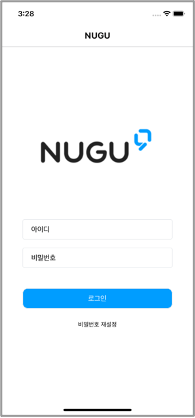
\includegraphics[width=3cm, height=6cm]{images/figure1.png}}
    \caption{Log-in}
    \end{figure}
    \begin{enumerate}
        \item Client could log-in with username\\
              Log-in through certified username. If certification is success, perform access token transmission.
        \item After log-in, user could see landing page.\\
    \end{enumerate}
    \item Landing
    \begin{figure}[htbp]
    \centerline{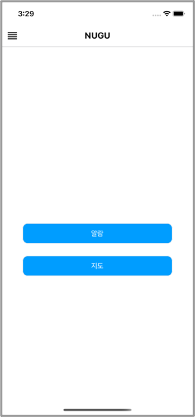
\includegraphics[width=3cm, height=6cm]{images/figure2.png}}
    \caption{Landing}
    \end{figure}
    \begin{enumerate}
        \item There are two options. One is alarm and The other is map.\\
    \end{enumerate}
    \item View kid’s notification
    \begin{figure}[htbp]
    \centerline{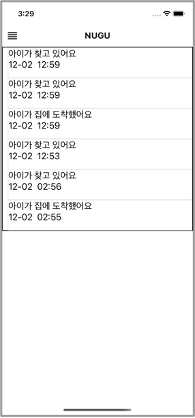
\includegraphics[width=3cm, height=6cm]{images/figure3.png}}
    \caption{Alarm}
    \end{figure}
    \begin{enumerate}
        \item Parent could see log list of the request by kids.
        \item “Kid is finding you” fixed message and timestamp will appear.
        \item “Kid arrive at home” fixed message and timestamp will appear.\\
    \end{enumerate}
    \item Set location of home and company 
    \begin{figure}[htbp]
    \centerline{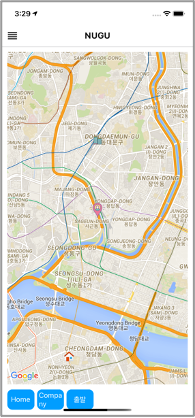
\includegraphics[width=3cm, height=6cm]{images/figure4.png}}
    \caption{Map}
    \end{figure}
    \begin{enumerate}
        \item Specify a specific location\\
              Use Google Map API’s function to search a specific location or return the current location. Set name the location and save it with latitude and longitude.
              \begin{enumerate}
                  \item location : varchar2(10)
                  \item latitude, longitude : float
              \end{enumerate}
        Ex) location :’회사’, latitude:36.232,\\
        longitude:35.231
        \item Add marker at the stored location
        \item Send user’s current location to server\\
        Use the background feature of the native app to send current location to server. Option for using location information must be checked by user before send this data.
    \end{enumerate}
\end{enumerate}

\subsection{Server}
\begin{enumerate}
    \item Judge parent’s location\\
    Server return different backend parameter depending on parent’s location.\\ \\
    -sudo code\\
    if CurrentLocation== KnownLocation\\
    return CurrentLocation, status\\
    //{location : ‘company’, status:’working’}\\
    elif CurrentLocation between KnownLocation\\
    and using RandomForest\\
    return KnownLocation, status\\
    //{location:[‘company’, ‘home’], status:’coming’}\\
    else\\
    return Status\\
    // {status : ‘외출 중’}\\ \\
    In between case, use ‘RandomForest’ model to predict status of parent based on location(longtitude, latitude) and timeStamp.
    
    \begin{enumerate}
        \item Get parent’s location data from application
        \begin{enumerate}
            \item Check latest location and judge status by customized algorithm.
            \item Response to NUGU.\\
        \end{enumerate}
    \end{enumerate}
    \item Send data to database
    \begin{enumerate}
        \item Server get data from NUGU speaker and application
        \item Server keep these data in database\\
    \end{enumerate}
    \item Make json for NUGU
    \begin{enumerate}
        \item Django Rest Framework module could handle this problem automatically.\\
    \end{enumerate}
\end{enumerate}

\section{Architecture Design}
\subsection{Overall Architecture}
Our service is web-based application and heavily depends on Amazon Web Service for deployment. Our application’s UI is implemented with React Native. Server is implemented by Python with Django framework web server on it to serve data to frontend UI as REST API, and interact with SKTelecom NUGU’s API and speaker. Entire API server is running on Amazon Web Service EC2 instance. Figure 1 shows overall architecture of the service.

\begin{figure}
    \centering
    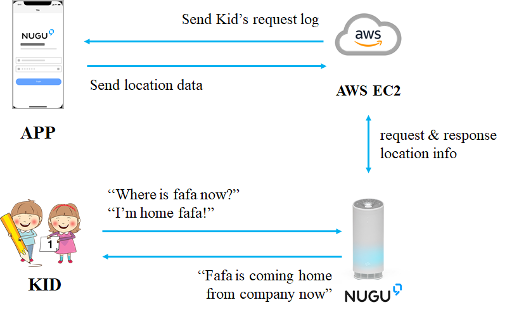
\includegraphics{images/figure5.png}
    \caption{Overall System Architecture Diagram}
\end{figure}

\subsection{NUGU Architecture Design}
Below are in-voice commands required to make interaction with SKTelecom NUGU Speaker.\\
\begin{enumerate}
    \item General Setting
    \begin{enumerate}
        \item Backend Proxy Server
        \item Web URL : TBA
        \item Exception message : “Connect Error”\\
    \end{enumerate}
    \item Intent
    \begin{enumerate}
        \item inform.home\\
        Inform to parent that kids get home now.\\
        Command : (FAMILY\_NAME), (ending of word) ex) “엄마 나 집왔어”
        
        \begin{table}[htbp]
        \begin{center}
        \caption{inform.home}
        \begin{tabular}{|c|c|c|}
        \hline
        \begin{tabular}[c]{@{}l@{}}Example\\ mention\end{tabular} & 엄마 & 나 집왔어 \\ \hline
        Category&FAMILY\_NAME  & ending of word \\ \hline
        Entity &FAMILY\_NAME  &STATEMENT\_HOME  \\ \hline
        \end{tabular}
        \end{center}
        \end{table}\\
        Action for inform home Intent : alert\_NUGU
        \begin{table}[htbp]
        \begin{center}
        \caption{alert\_NUGU}
        \begin{tabular}{|c|c|c|c|}
        \hline
        \begin{tabular}[c]{@{}l@{}}Example\\ mention\end{tabular} & 엄마 & 에게 &\begin{tabular}[c]{@{}l@{}}집에 왔다고\\ 알려드렸어요\end{tabular} \\ \hline
        Category&FAMILY\_NAME  & Postposition&Ending of word\\ \hline
        \begin{tabular}[c]{@{}l@{}}Utterance\\ Parameter\end{tabular} &FAMILY\_NAME  &Fixed postposition& Fixed statement \\ \hline
        \end{tabular}
        \end{center}
        \end{table}\\
        \item ask.location\\
        Ask for family’s location\\
        Command : (FAMILY\_NAME), (ending of word) \\ex) 엄마 어디야?
        \begin{table}[htbp]
        \begin{center}
        \caption{ask.location}
        \begin{tabular}{|c|c|c|}
        \hline
        \begin{tabular}[c]{@{}l@{}}Example\\ mention\end{tabular} & 엄마 & 어디야? \\ \hline
        Category&FAMILY\_NAME  & ending of word \\ \hline
        Entity &FAMILY\_NAME  &STATEMENT\_HOME  \\ \hline
        \end{tabular}
        \end{center}
        \end{table}\\
        Action for ask.location Intent
        \begin{enumerate}
            \item now\_location\\
            When family member is in designated place, now\_location tells the location of family member.
            \begin{table}[htbp]
            \begin{center}
            \caption{now\_location}
            \begin{tabular}{|c|c|c|c|c|}
            \hline
            \begin{tabular}[c]{@{}l@{}}Example\\ mention\end{tabular} & 엄마&는&회사&에 있어요 \\ \hline
            Category&\begin{tabular}[c]{@{}l@{}}FAMILY\\ \_NAME \end{tabular} & Postposition& Location&\begin{tabular}[c]{@{}l@{}}Ending \\of word \end{tabular}\\ \hline
            \begin{tabular}[c]{@{}l@{}}Utterance\\ Parameter\end{tabular}&\begin{tabular}[c]{@{}l@{}}FAMILY\\ \_NAME \end{tabular}&\begin{tabular}[c]{@{}l@{}}Fixed\\ post position\end{tabular}&LOCATION&
            \begin{tabular}[c]{@{}l@{}}Fixed\\ Statement\end{tabular}\\ \hline
            \end{tabular}
            \end{center}
            \end{table}
            
            \item between\_location \\
            When family member is between home and company, between\_location tells the starting point, destination, and status.
            
            \begin{table}[htbp]
            \begin{center}
            \caption{between\_location}
            \begin{tabular}{|c|c|c|c|c|}
            \hline
            \begin{tabular}[c]{@{}l@{}}Example\\ mention\end{tabular} & 엄마&는&회사&에서 \\ \hline
            Category&\begin{tabular}[c]{@{}l@{}}FAMILY\\ \_NAME \end{tabular} & Postposition& Location&Postposition\\ \hline
            \begin{tabular}[c]{@{}l@{}}Utterance\\ Parameter\end{tabular}&\begin{tabular}[c]{@{}l@{}}FAMILY\\ \_NAME \end{tabular}&\begin{tabular}[c]{@{}l@{}}Fixed\\ post position\end{tabular}&\begin{tabular}[c]{@{}l@{}}START\_ \\LOCATION\end{tabular}&
            \begin{tabular}[c]{@{}l@{}}Fixed\\ Statement\end{tabular}\\ \hline
            \end{tabular}
            \end{center}
            \end{table}
            \begin{table}[htbp]
            \begin{center}
            \begin{tabular}{|c|c|c|c|}
            \hline
            집&으로&퇴근하는&중이에요 \\ \hline
            Location&Postposition & Status&\begin{tabular}[c]{@{}l@{}}Ending \\of word \end{tabular} \\ \hline
            DESTI\_LOCATION&Fixed postposition&STATUS&\begin{tabular}[c]{@{}l@{}}Fixed \_ \\Statement\end{tabular}\\ \hline
            \end{tabular}
            \end{center}
            \end{table}
            
            \item except\_location \\
            When family member is not in designated place and not between two designated places, except\_location tells family member is gone.
            
            \begin{table}[htbp]
            \begin{center}
            \caption{except\_location}
            \begin{tabular}{|c|c|c|c|}
            \hline
            \begin{tabular}[c]{@{}l@{}}Example\\ mention\end{tabular} & 엄마&는&
            지금 외출 중이에요 \\ \hline
            Category&\begin{tabular}[c]{@{}l@{}}FAMILY\_NAME \end{tabular} & Postposition& Statement\\ \hline
            \begin{tabular}[c]{@{}l@{}}Utterance\\ Parameter\end{tabular}&\begin{tabular}[c]{@{}l@{}}FAMILY\_NAME \end{tabular}&\begin{tabular}[c]{@{}l@{}}Fixed\\ post position\end{tabular}&
            \begin{tabular}[c]{@{}l@{}}Fixed Statement\end{tabular}\\ \hline
            \end{tabular}
            \end{center}
            \end{table}\\
        \end{enumerate}
    \end{enumerate}
   \item Entity
   \begin{enumerate}
       \item FAMILY\_NAME\\Family members
       \begin{table}[htbp]
       \begin{center}
       \caption{FAMILY\_NAME}
       \begin{tabular}{|c|c|}
       \hline
       Parameter & Synonym \\ \hline
       엄마        & 어머니     \\ \hline
       아빠        & 아버지     \\ \hline
       형         & 오빠, 형님  \\ \hline
       누나        & 언니      \\ \hline
       \end{tabular}
       \end{center}
       \end{table}
       \item STATEMENT\_HOME\\Fixed Statement for ending of word when kid come back 
       \begin{table}[htbp]
       \begin{center}
       \caption{STATEMENT\_HOME}
       \begin{tabular}{|c|c|}
       \hline
       Parameter & Synonym                    \\ \hline
       나 집이야     & 나 지금 집이야, 나 도착했어, 나 집왔어... \\ \hline
       \end{tabular}
       \end{center}
       \end{table}
       
       \item STATEMENT\_LOCATION\\
       Fixed Statement for ending of word when kid ask for family member’s location.
        \begin{table}[htbp]
        \begin{center}
        \caption{STATEMENT\_LOCATION}
       \begin{tabular}{|c|c|}
       \hline
       Parameter & Synonym                    \\ \hline
       어디야     & 어디야, 지금 어디야, 어디에요, 지금 어디에요... \\ \hline
       \end{tabular}
       \end{center}
       \end{table}
   \end{enumerate}
   
   \item Actions
   \begin{enumerate}
       \item alert\_NUGU
       \begin{enumerate}
           \item Custom Action
           \item Using it when kid come back home
           \item Trigger
           \item inform.home \\ Ex) “엄마, 나 도착했어”
           \item Prompt \\ Ex) “{{FAMILY\_NAME
           \_}}에게 집에 왔다고 알려 드렸어요.”
       \end{enumerate}
       \item location
       \begin{enumerate}
           \item Custom Action
           \item Root Action
           \item Trigger: ask.location
           \item Output
           \begin{itemize}
               \item now\_location\\
               - Branch Action\\
               - Using it when family member is in designated place.\\
               - Trigger: When LOCATION(Backend Parameter) exist\\
               - Prompt\\
               Ex)”{{FAMILY\_NAME}}은 {{LOCATION}}에 있어요”\\
               \item between\_location\\
               - Branch Action\\
               - Using it when family member is going to designated place or home.\\
               - Trigger: When START\_LOCATION and DESTI\_LOCATION(Backend Parameter) exist.\\
               - Prompt\\
               Ex)“{{FAMILY\_NAME}}는 {{START\_LOCATION}}에서 {{DESTI\_LOCATION}}으로 {{STATUS}} 중이에요”\\
                \item except\_location\\
                - Branch Action\\
                - Using it when family member is not in designated place or not between two designated places.\\
                - Prompt\\
                Ex) “{{FAMILY\_NAME}}은 지금 외출 중이에요.” \\
           \end{itemize}
       \end{enumerate}
   \end{enumerate}
\end{enumerate}

\subsection{Database Design}
\begin{figure}[htbp]
    \centering
    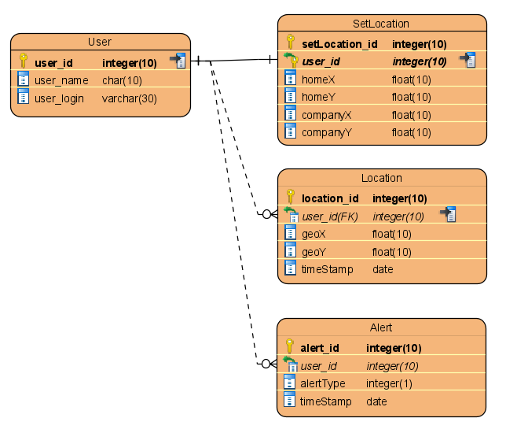
\includegraphics{images/figure6.png}
    \caption{Database Design}
\end{figure}
\begin{enumerate}
    \item User
    \begin{enumerate}
        \item user\_id(PK) : identification of user
        \item user\_name : user’s name
        \item user\_log-in : information of user log-in(like token)\\
    \end{enumerate}
    
    \item SetLocation
    \begin{enumerate}
        \item setLocation\_id(PK) : identification of SetLocation
        \item user\_id(FK) : reference ‘User’ table \\
	    one user could set only one home and company
	    \item homeX : longtitude of user’s home
	    \item homeY : latitude of user’s home
	    \item companyX : lontitude of user’s company
	    \item companyY : latitude of user’s company\\
    \end{enumerate}
    
    \item Location
    \begin{enumerate}
        \item location\_id(PK) : identification of Location
        \item user\_id(FK) : reference ‘User’ table\\
	    one user could make multiple location logs
        \item geoX : lontitude of user
        \item geoY : latitude of user
        \item timeStamp : time of this data made
    \end{enumerate}
    
    \item Alert
    \begin{enumerate}
        \item alert\_id(PK) : identification of Alert
        \item user\_id(FK) : reference ‘User’ table \\
	    one user could make multiple alert logs
	    \item alertType : define what request is this
	    \item timeStamp : time of this data made\\
    \end{enumerate}
\end{enumerate}

\subsection{Directory Organization – Front End}
Table 14 shows the directory organization of React-Native frontend application’s project.
\begin{table}[htbp]
\begin{center}
\begin{tabular}{|c|c|c|}
\hline
Directory & File names & Module name in use \\ \hline
/src/components & Index.tsx & styled-components/native\\ \hline
/src/Assets/Images & .png &-\\ \hline
/src/Screens/Navigator & Index.tsx & react-navigation\\ \hline
/src/Screens/Log-in & Index.tsx &\begin{tabular}[c]{@{}c@{}} react-native-community/\\async-storage  \end{tabular}                    \\ \hline
 /src/Screens/CheckLogin & Index.tsx& \begin{tabular}[c]{@{}c@{}} react-native-community/\\async-storage  \end{tabular} \\ \hline
 /src/Screens/Map & Index.tsx & \begin{tabular}[c]{@{}c@{}} react-native-maps, \\react-native-geolocation-service
  \end{tabular}                   \\ \hline
\end{tabular}
\end{center}
\end{table}

\begin{enumerate}
    \item /src/components\\
    React-native uses functional-component-based development method. This folder contains components that are frequently used like button, Input components. We will use these components by export and import function.\\
    \item /src/Assets/Images\\
    Inside the Asset folder, there are resources such as image files and fonts needed for the application. There are app icons, button images, and marker images in the image folder images.\\
    \item /src/Assets/Screens\\
    The Screens folder contains functions that make up the screens in the application. Navigator is a function that controls the movement of the screen. The screen consists of a Log-in screen for log-ins, a CheckLogin screen for tokens checking, and a Map window for positioning.\\
    \item styled-components/native\\
    Styled Components is an open-source library that helps with the application of styling of react and react native. It can create a style on a single JavaScript file. In other words, you can do CSS work in JavaScript files without CSS files.\\
    \item react-navigation\\
    A React Navigation is a chain of navigators that define the screen flow of your app. React Navigation's stack navigator provides a way for your app to transition between screens and manage navigation history.\\
    \item react-native-community/async-storage\\
    React Native Async Storage is an asynchronous, unencrypted, persistent, key-value storage system for React Native. Async Storage send and receive data like token, user information, location of home and company with Backend Server.\\
    \item react-native-geolocation-service\\
    React Native Geolocation Service tell user’s current location and allows to track user’s location. Using this module, we took user’s current location and whenever the user’s location changed, we used fetch module to send the location information to backend server.\\
    \item react-native-maps\\
    React Native Maps is a component system for maps. Using this module, we displayed Google Maps on the screen and marked house, company, user’s current location with marker\\
\end{enumerate}

\subsection{Directory Organization – Back End}
\begin{table}[htbp]
\begin{center}
\caption{DIRECTORY ORGANIZATION FOR\\ BACKEND APPLICATION PROJECT}
\begin{tabular}{|c|c|c|}
\hline
Directory & File names & Module name in use \\ \hline
/.ebextensions & django.config &\begin{tabular}[c]{@{}l@{}}  Django, AWS\\ ElasticBeanstalk\end{tabular}  \\ \hline
/.elasticbeanstalk &config.yml & AWS ElasticBeanstalk \\ \hline
 /NUGU &  settings.py, urls.py, wsgi.py  & \begin{tabular}[c]{@{}l@{}} Django,\\ Django RestFramework\end{tabular}\\ \hline
 /FAFA & \begin{tabular}[c]{@{}l@{}}models.py, serializers.py,\\ urls.py, views.py\end{tabular} & \begin{tabular}[c]{@{}l@{}} Django,\\ Django RestFramework\end{tabular} \\ \hline
/static & .css, .js, .img&  -              \\ \hline
  -        &\begin{tabular}[c]{@{}l@{}}.gitignore, db.sqlite3,\\ manage.py, requirements.txt\end{tabular}&Django\\ \hline
\end{tabular}
\end{center}
\end{table}
\begin{enumerate}
    \item /.ebextensions\\
    In order to implement Django module on AWS ElasticBeanstalk environment, path configuration needed. ‘django.config’ file contains option for setting and covers deploy problem.\\
    \item /.elasticbeanstalk\\
    To upload directory on AWS instance, application name or region and the other configuration needed. ‘config.yml’ would cover upload problem.\\
    \item /NUGU\\
    In order to use Django framework which is run by Python, allowed hosts, url, apps, packages and other things should be set on this directory. On ‘settings.py’ and ‘urls.py’ files, there are some customized setting for this project.\\
    \item /FAFA\\
    Django RestFramework module is used in this directory. ‘models.py’ make models (DB table). ‘urls.py’ handles routing. ‘views.py’ gets request and sends response by function that we made. ‘serializers.py’ make response in json form from queryset.\\
    \item SQLite\\
    SQLite is relatively light embedded database for applications. To store data, only one file ‘db.sqlite3’ is needed. Small and concise DB would run in local, so you don’t have to worry about the cost of network configuration, firewalls, network address translation, and so on. We can only focus on code level.\\
    \item AWS ElasticBeanstalk\\
    A fully managed service of AWS that deploy, expand and manage web application. It handles capacity provisioning, load balancing, auto scaling, monitoring, and hosting environment automatically. So user just deploy application. In addition, there is no unnecessary expenditure to pay. Through easy deployment, this module makes us focus on code level during development. \\
    \item Django\\
    Django is Web framework used in our project. Using this module, we don’t ‘reinvent the wheel’ about HTTP service. Django provide simple and convenient middle-ware like routing, error-handler and parser. Many of above middle-ware can be implemented in custom way that we want to make.\\
    \item Django Rest Framework(DRF)\\
    DRF is a powerful and flexible module for creating WEB APIs. To develop backend proxy server of NUGU-PLAY in REST API form, we used DRF. This module has powerful ‘viewset’ that enables us to develop CRUD functions easily and quickly. Also we can customize a general view. 
\end{enumerate}

\section{Use Cases}
FAFA service is used by kids and parents. Kids use our service via NUGU speaker, Parents use our service throguh application that we developed in React Native. Application and NUGU speaker are connected by backend proxy server which is developed in REST API format by Django framework. Under Diagram shows flow of our service and algorithm that how to define parent’s status based on location data.\\

\begin{figure*}[htbp]
        \centering
        \hfill
        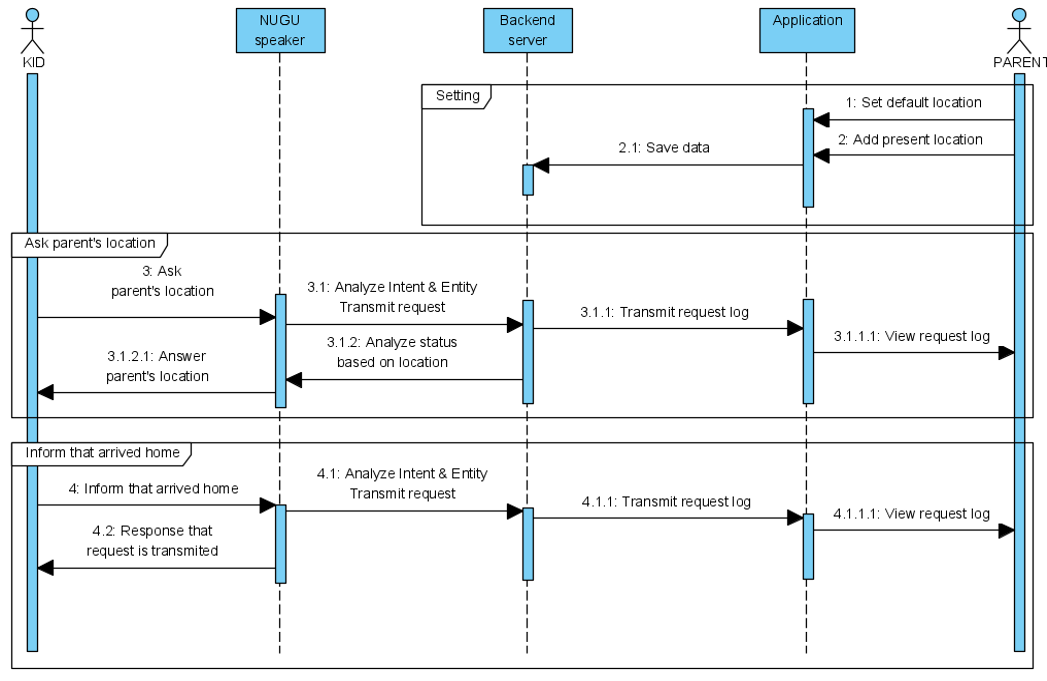
\includegraphics[width=\textwidth, height=10cm]{images/figure7.png}
        \hfill
        \caption{Sequence diagram}
\end{figure*}
    
\begin{figure}[htbp]
        \centering
        \hfill
        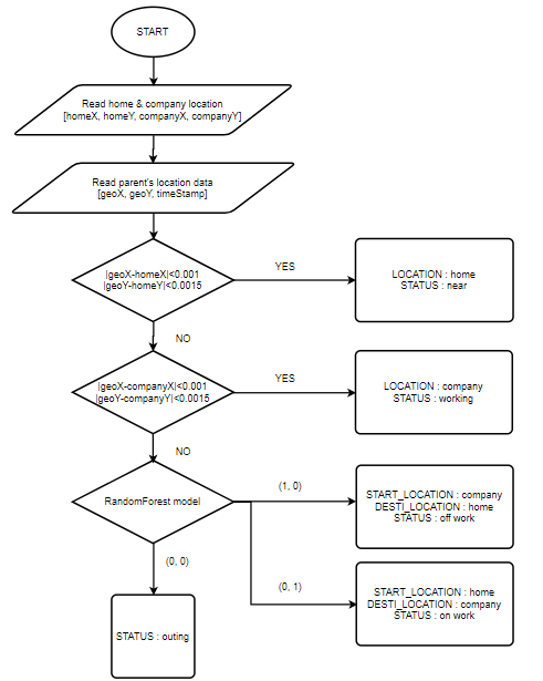
\includegraphics[height=10cm]{images/figure8.png}
        \hfill
        \caption{Flow of ‘Anlayze parent’s status based on location’}
\end{figure}

\begin{enumerate}
    \item NUGU speaker\\
    Depending on above algorithm which is using randomForest model to define that parents are coming or going, There are 3 answers when kids ask parent’s location through NUGU speaker. In addition, there is fixed response when inform to speaeker that kids arrived home.
    \begin{enumerate}
        \item “Parent is working in office” by speaker\\
        If parent’s latest location is near to home or office, NUGU speaker tells to kids “Mom is working in office” or “Fafa is near home”. Figure 10 explains this logic. 0.001 longtitude means 100 meter and 0.0015 longtitude means 100 meter.\\
        \item “Parent is coming home from office now” by speaker\\
        We predict parent’s status by using randomForest which is one of Machine Learning method. Train data is saved automatically by application that we made. If kids ask parent’s location, backend server puts parent’s latest location on randomForest model and judge that parents are coming or going home.\\
        \item “Parent is out now” by speaker\\
        If parent’s latest location is out of boundary between home and company. NUGU speaker says “Parent is out now”\\
        \item “Told to parents that you arrived home now” by speaker\\
        If kids inform that they arrived home now, NUGU speaker sends this log to backend server and response above message.\\
    \end{enumerate}
\end{enumerate}
\subsection{Application}
\begin{enumerate}
    \item Log-in\\
    When user access our application, They have to log-in by  ID and Password. To use NUGU speaker, they need to log in with their T ID.\\
    \begin{figure}[htbp]
        \centering
        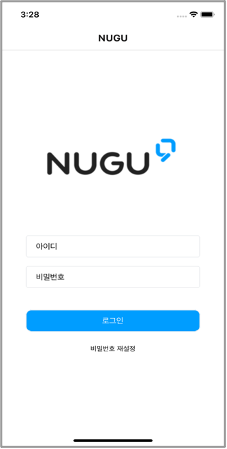
\includegraphics[width=3cm, height=6cm]{images/figure9.png}
        \caption{Log-in}
    \end{figure}
    
    \item Landing\\
    When user log-in to our application, the landing screen is on. There are two options. One is an alarm page that shows alarm and the other is a map page that track user’s location.\\
    \begin{figure}[htbp]
        \centering
        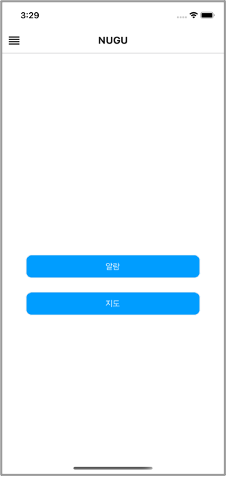
\includegraphics[width=3cm, height=6cm]{images/figure10.png}
        \caption{Landing}
    \end{figure}
    
    \item Alarm\\
    This page shows thar when the child found his parents and when the child arrived home. It informs user of alarm and the time the alarm came.
    \begin{figure}[htbp]
        \centering
        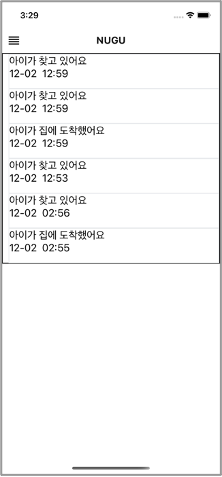
\includegraphics[width=3cm, height=6cm]{images/figure11.png}
        \caption{Alarm}
    \end{figure}
    
    \item Check current location\\
    User can check his current location by Google Map. When user click list button on the upper left corner, user can return to landing screen.
    \begin{figure}[htbp]
        \centering
        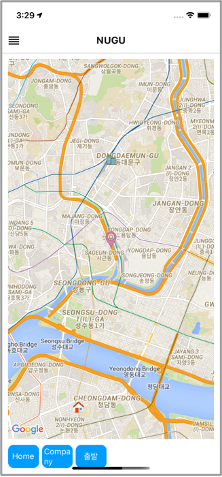
\includegraphics[width=3cm, height=6cm]{images/figure12.png}
        \caption{Check current Location}
    \end{figure}
    
    \item Indicate that user is going home\\
    When clicking start button, user tell server that user is on user’s way home. The Start button changes to the arrival button. When the user arrives home, press the arrival button.\\
    \begin{figure}[htbp]
        \centering
        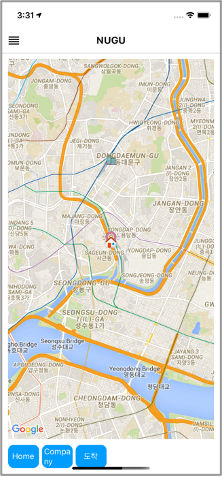
\includegraphics[width=3cm, height=6cm]{images/figure13.png}
        \caption{Indicate that user is going home}
    \end{figure}
    \\
    
    
    \item Location Tracking\\
    Whenever the user’s location changes by more than 100 meters, the location information is sent to the server and displayed on the screen.\\
    \begin{figure}[htbp]
        \centering
        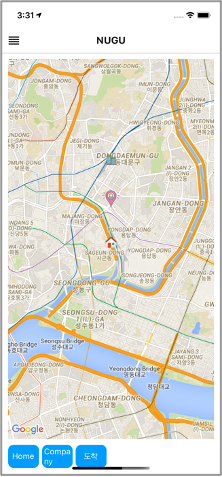
\includegraphics[width=3cm, height=6cm]{images/figure14.png}
        \caption{Location Tracking}
    \end{figure}
     \\
    \item Sending Data for AI’s Learning\\
    The server analyze the location information through AI and predict the way home. So when enough data is accumulated, it determines whether you are one your way home without pressing start button.\\
    \item Set Home Location\\
    When the User press the home button, the current location is set to the home position and a home icon is created.
    \begin{figure}[htbp]
        \centering
        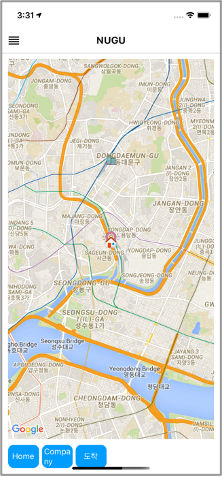
\includegraphics[width=3cm, height=6cm]{images/figure15.png}
        \caption{Set Home Location}
    \end{figure}
    
    \item Set Company Location\\
    When the User press the company button, the current location is set to the company position and a company icon is created.
    \begin{figure}[htbp]
        \centering
        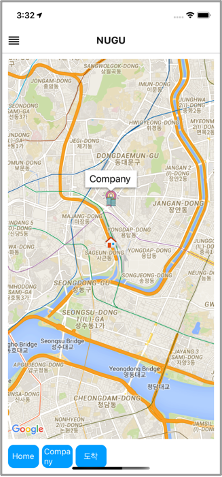
\includegraphics[width=3cm, height=6cm]{images/figure16.png}
        \caption{Set Company Location}
    \end{figure}
    
    
\end{enumerate}

\end{document}
